\documentclass[a4paper]{article}
\usepackage[utf-8]{inputenc}
\usepackage[spanish]{babel}
\usepackage{graphicx}
\usepackage{float}

\begin{document}

{\large Perfilador de haz}

\section{Especificaciones}

\begin{figure}[H]
  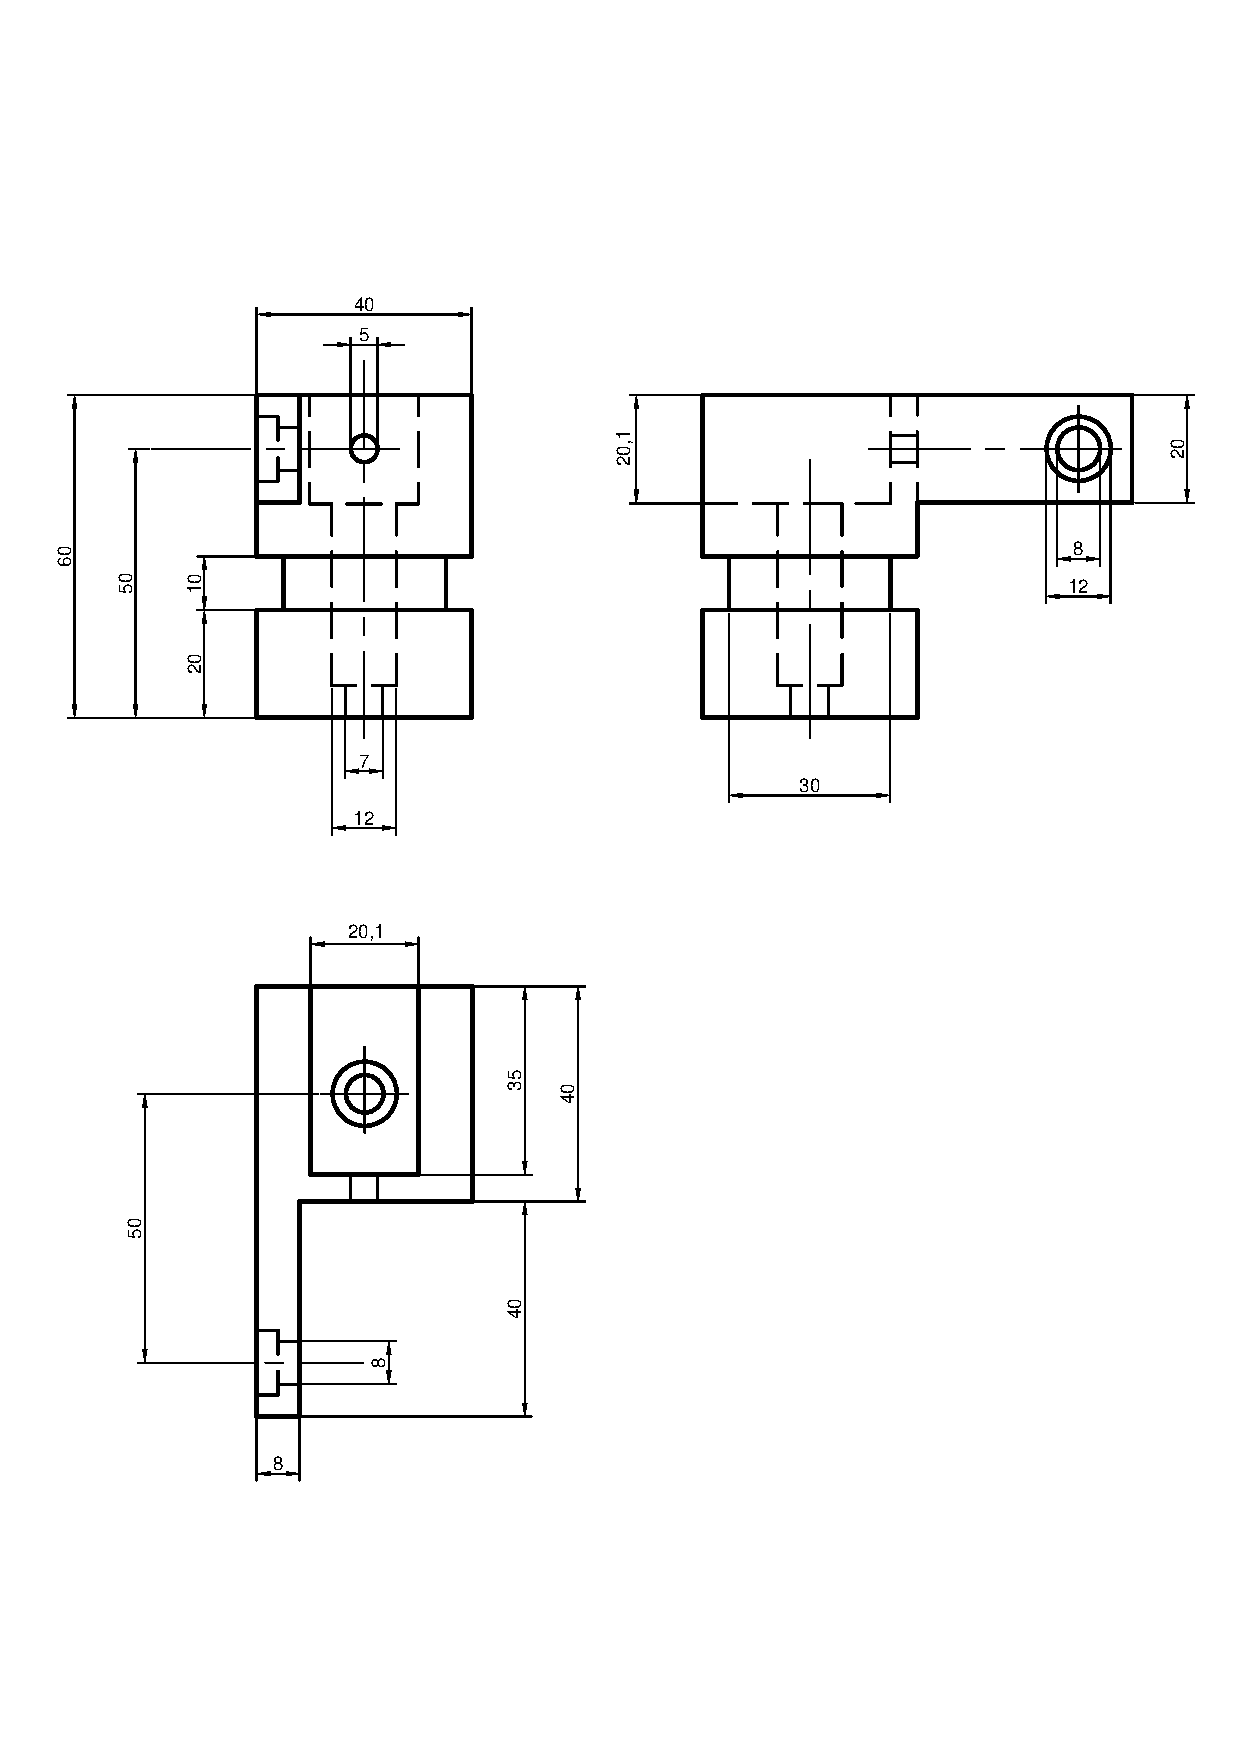
\includegraphics[width=0.5\textwidth]{mecanica.pdf}
  \label{fig:mecanica}
  \caption{Esquema mecánico del perfilador}
\end{figure}

El diseño del perfilador permite medir un haz teniendo en cuenta
\begin{itemize}
  \item Diametro máximo de haz perfilable: 10 mm
  \item Altura del eje óptico respecto al plano de apoyo: 5 cm
  \item Distancia del agujero del soporte al eje óptico: 7.5 cm
\end{itemize}

Esto permite medir en los siguientes setups
\begin{itemize}
  \item Riel Tholabs. En el eje vertical sin agregados, en otro eje con un poste Thorlabs
  \item Cage de Thorlabs de 30mm y 60mm. Posible necesidad de soporte por la altura del eje
  \item Con un poste y un soporte agujereado de Thorlabs puede ubicarse a cualquier altura y setup
\end{itemize}

\subsection{Electrónica de adquisición y software}
Con la velocidad del motor y la velocidad de la electrónica se dispone la siguiente velocidad de adquisición
\begin{itemize}
  \item 40 perfiles por segundo
\end{itemize}



\end{document}
